% Filename: chap01@camecc_lic.tex
% This code is part of 'Cursos CAMECC: Introducao ao LaTeX para o Curso 29 - Licenciatura em Matematica'
% 
% Description: This file correspond to the chapter 01 of the textbook using in the course.
% 
% Created: 07.06.12 11:30:49 AM
% Last Change: 07.06.12 11:30:53 AM
% 
% Authors:
% - Raniere Silva, r.gaia.cs@gmail.com
% 
% Organization: CAMECC - Centro Academico dos Estudantes do IMECC
% 
% Copyright (c) 2012, Raniere Silva. All rights reserved.
% 
% This work is licensed under the Creative Commons Attribution-ShareAlike 3.0 Unported License. To view a copy of this license, visit http://creativecommons.org/licenses/by-sa/3.0/ or send a letter to Creative Commons, 444 Castro Street, Suite 900, Mountain View, California, 94041, USA.
%
% This work is distributed in the hope that it will be useful, but WITHOUT ANY WARRANTY; without even the implied warranty of MERCHANTABILITY or FITNESS FOR A PARTICULAR PURPOSE.
%
\chapter{Ol\'{a} \LaTeX}
Neste primeiro cap\'{i}tulo apresentamos os conhecimementos m\'{i}nimos de todo usu\'{a}rio do LaTeX. Os cap\'{i}tulos~\ref{sch:history}~e~\ref{sch:get_help} s\~{a}o uma complementa\c{c}\~{a}o a este cap\'{i}tulo podendo ser lidos de maneira independente.

\section{Instala\c{c}\~{a}o}\index{instalacao@instala\c{c}\~{a}o}
Para utilizar o LaTeX voc\^{e} precisa das macros que comp\~{o}em o LaTeX, disponiveis para
\begin{itemize}
    \item Linux: TeX Live\index{TeX Live|see{instala\c{c}\~{a}o}} (\url{http://www.tug.org/texlive}),
    \item Mac OS X: MacTeX\index{Mac OS X|see{instala\c{c}\~{a}o}} (\url{http://www.tug.org/mactex/}),
    \item Windows: proTeXt\index{proTeXt|see{instala\c{c}\~{a}o}} (\url{http://www.tug.org/protext/}) ou MiKTeX\index{MikTeX|see{instala\c{c}\~{a}o}} (\url{http://www.miktex.org/}),
\end{itemize}
e de um editor de texto. \'{E} recomendado que ao inv\'{e}s de um editor de texto utilize-se uma IDE\index{IDE} (\flang{Integrated Development Environment}) pr\'{o}pria para o LaTeX, como
\begin{itemize}
    \item TeXworks\index{TeXworks|see{IDE}} (\url{http://www.leliseron.org/texworks/}),
    \item Kile\index{Kile|see{IDE}} (\url{http://kile.sourceforge.net/}),
    \item Texmaker\index{Texmaker|see{IDE}} (\url{http://www.xm1math.net/texmaker/}).
\end{itemize}
O TeXworks costuma acompanhar a maioria das distribui\c{c}\~{o}es do LaTeX e por isso ser\'{a} utilizado neste curso. Uma lista com v\'{a}rias IDE's encontra-se dispon\'{i}vel em \url{http://en.wikipedia.org/wiki/Comparison_of_TeX_editors}\nocite{Wikipedia:EN:Comparison_TeX_editors} e imagens de algumas delas s\~{a}o apresentadas na Figura~\ref{fig:ide_screenshot}.
\begin{figure}[!htb]
    \centering
    \begin{tabular}{cc}
        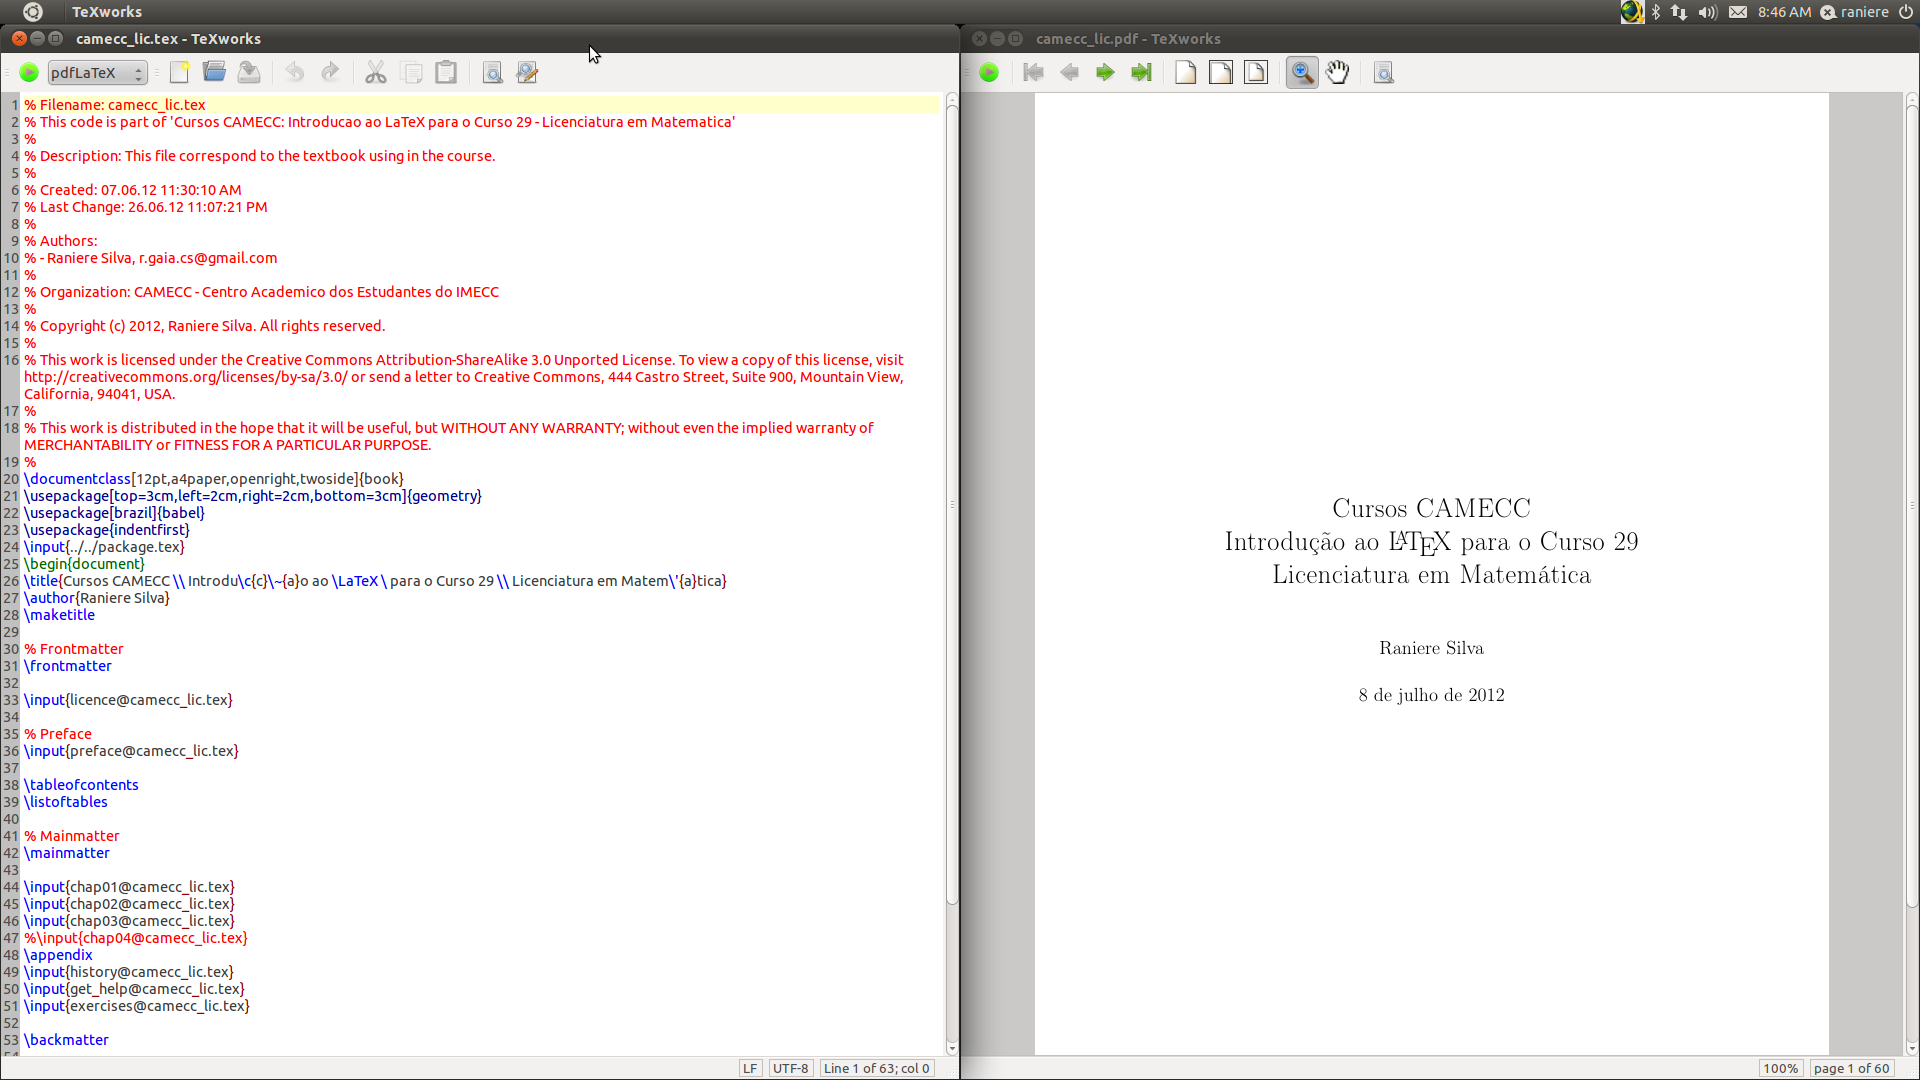
\includegraphics[width=0.4\textwidth]{../../figures/texworks.png} &
        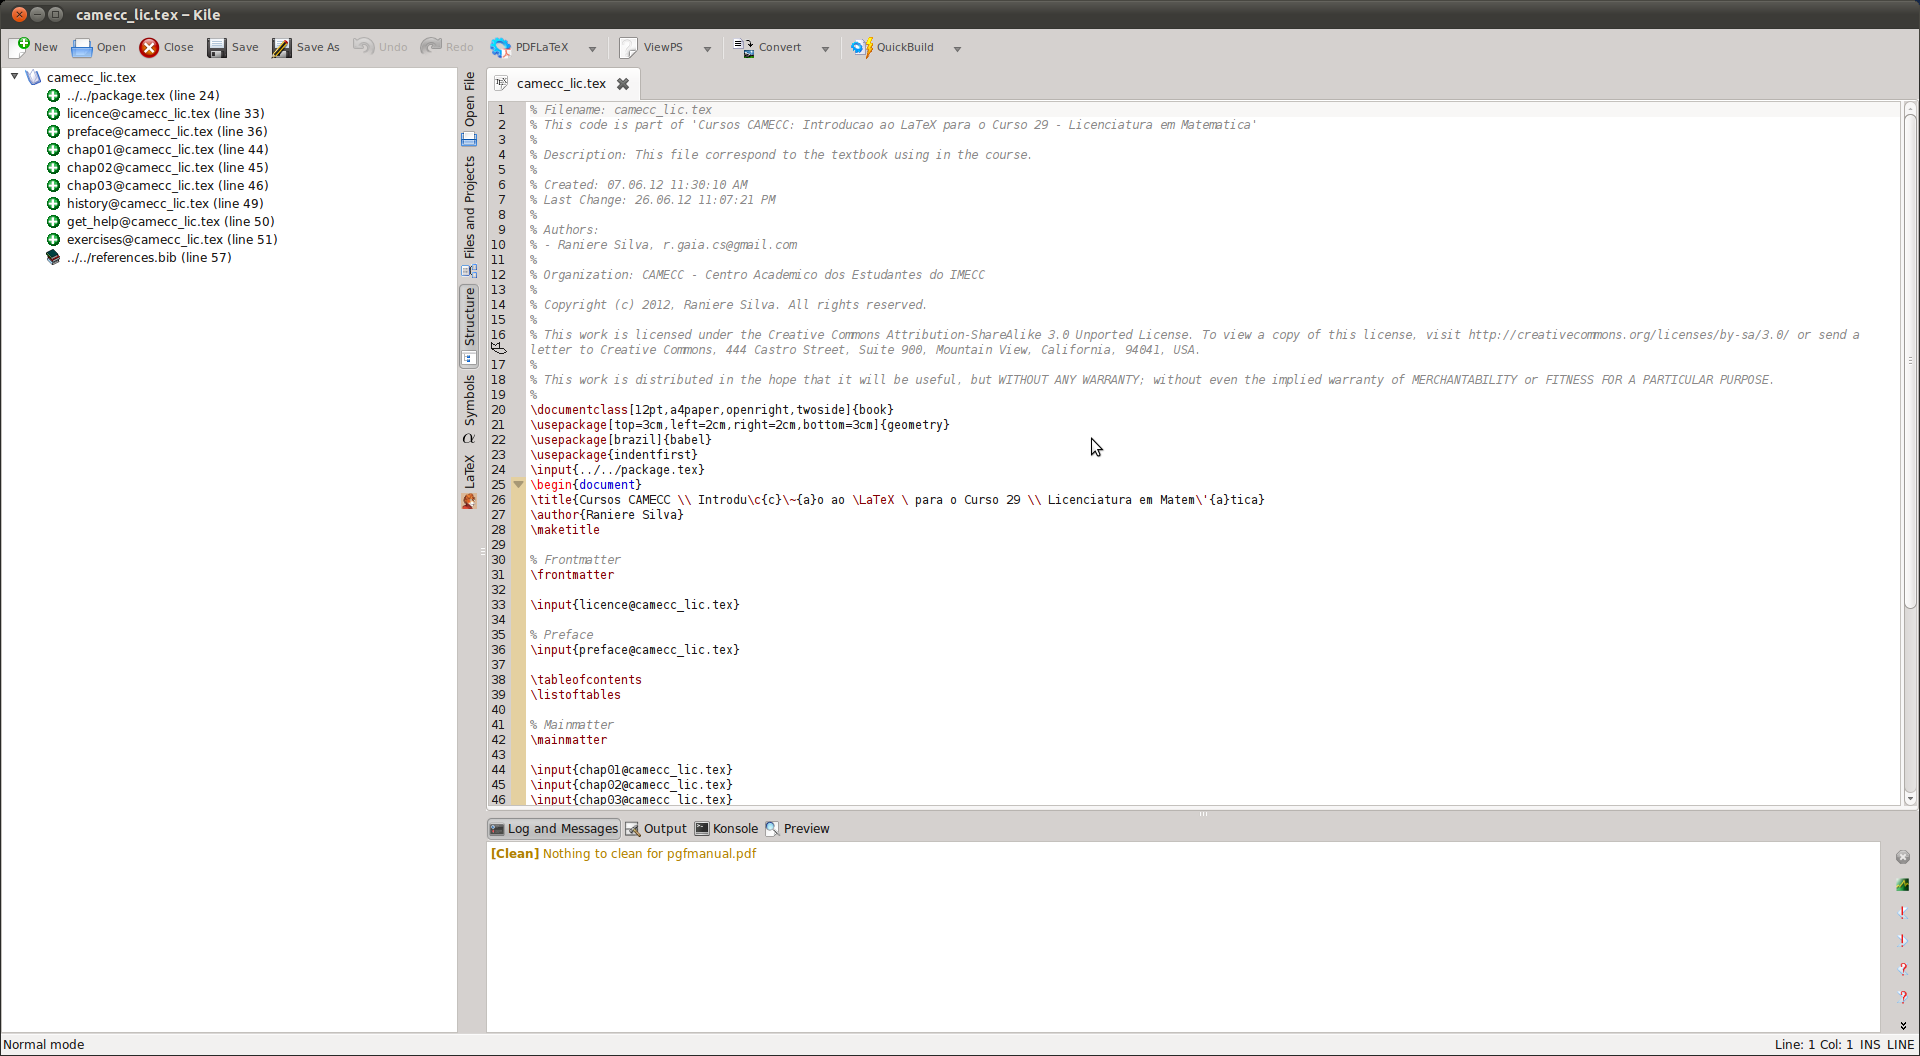
\includegraphics[width=0.4\textwidth]{../../figures/kile.png} \\
        Texworks & Kile \\
        % 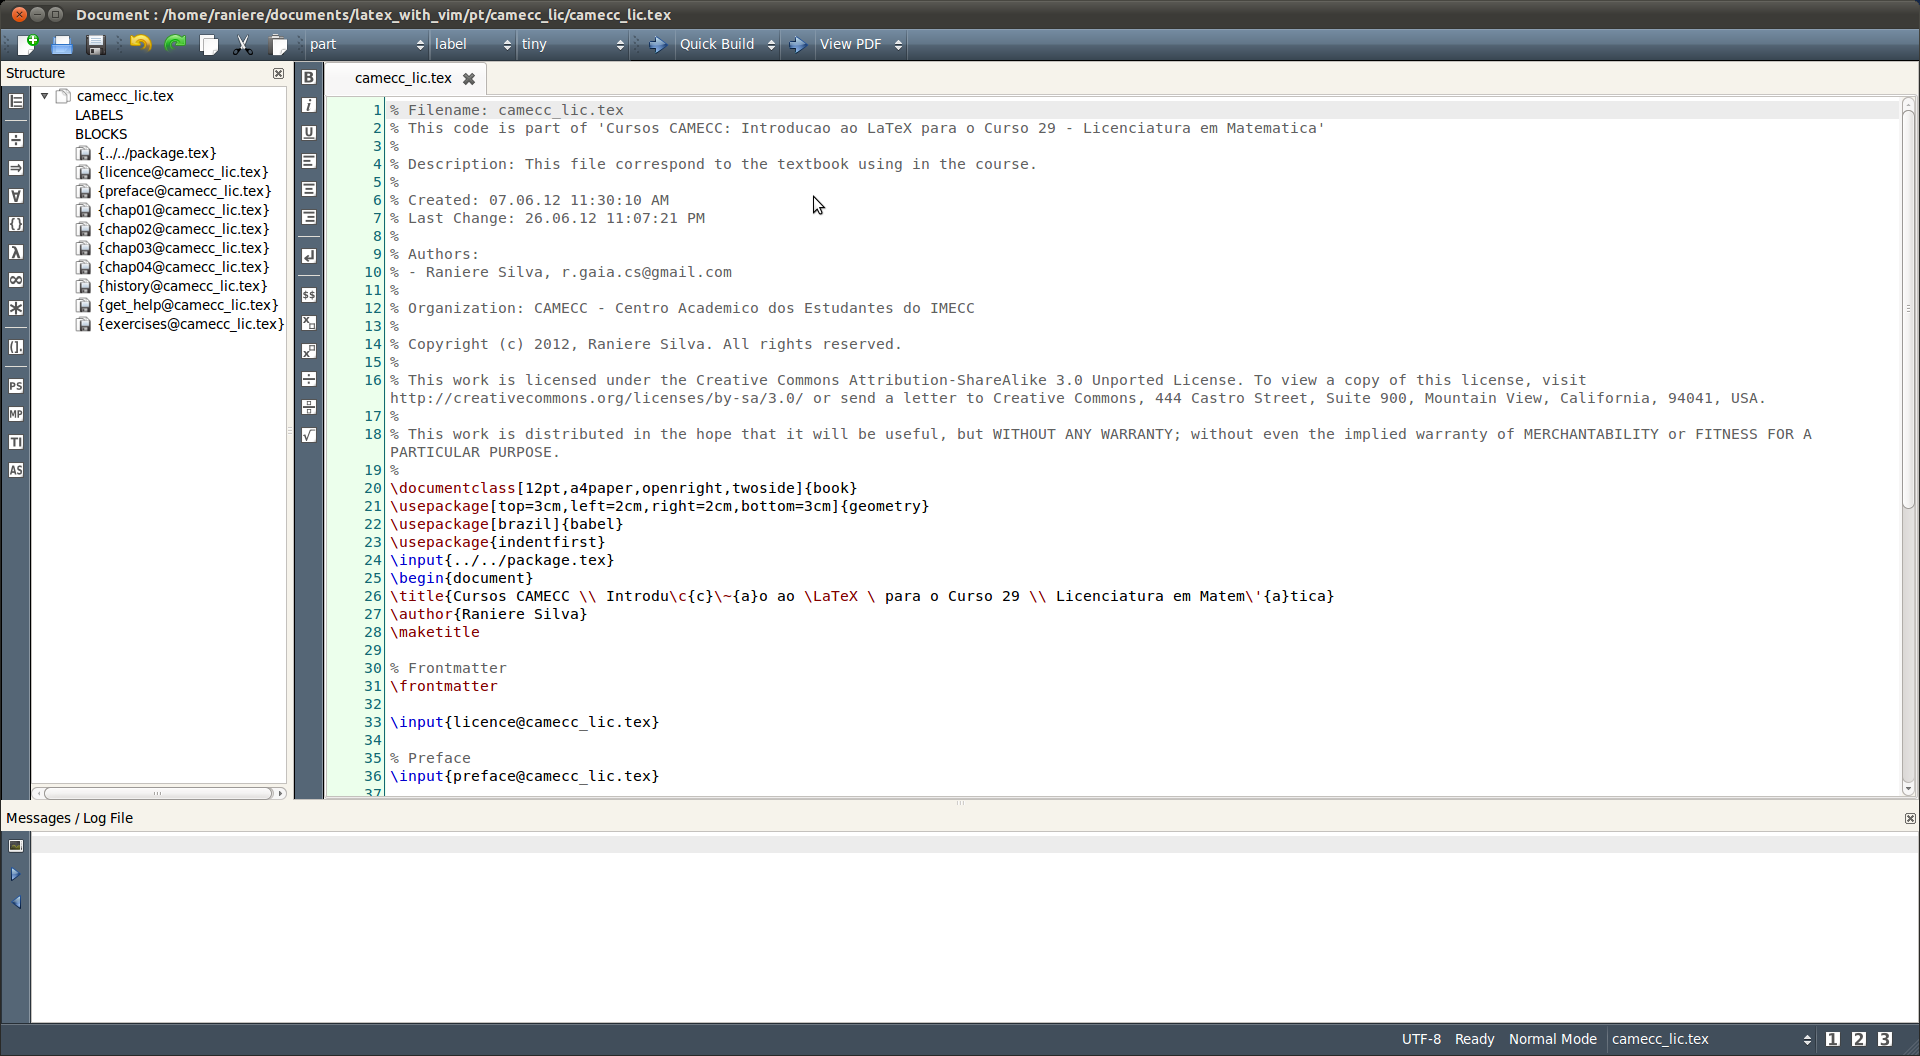
\includegraphics[width=0.4\textwidth]{../../figures/texmaker.png} &
        % 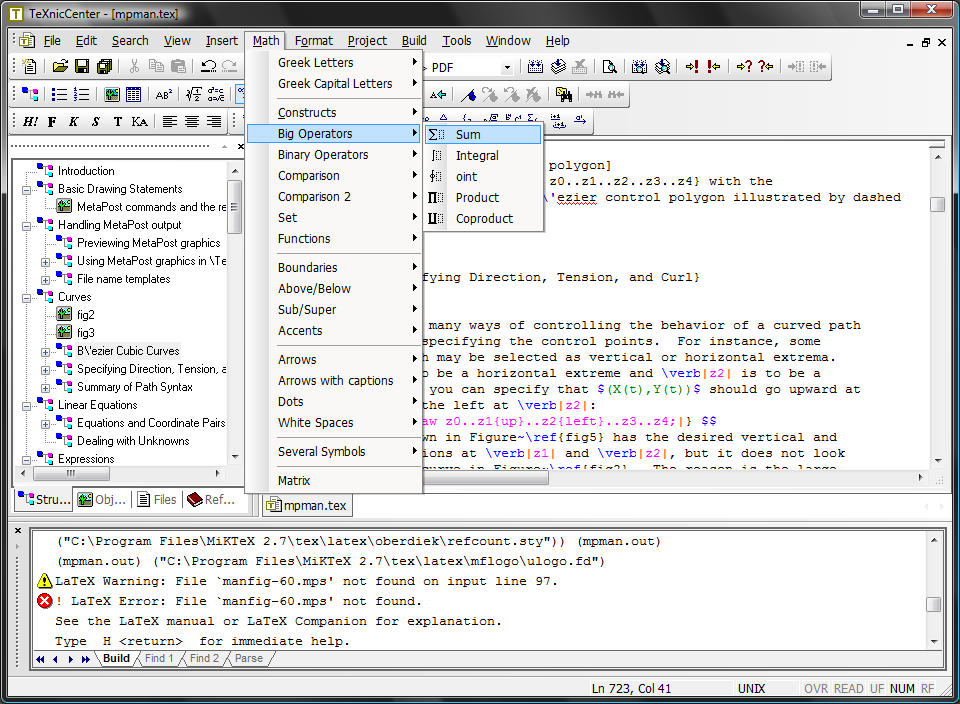
\includegraphics[width=0.4\textwidth]{../../figures/texniccenter.png} \\
        % Texmaker & TexnicCenter \\
        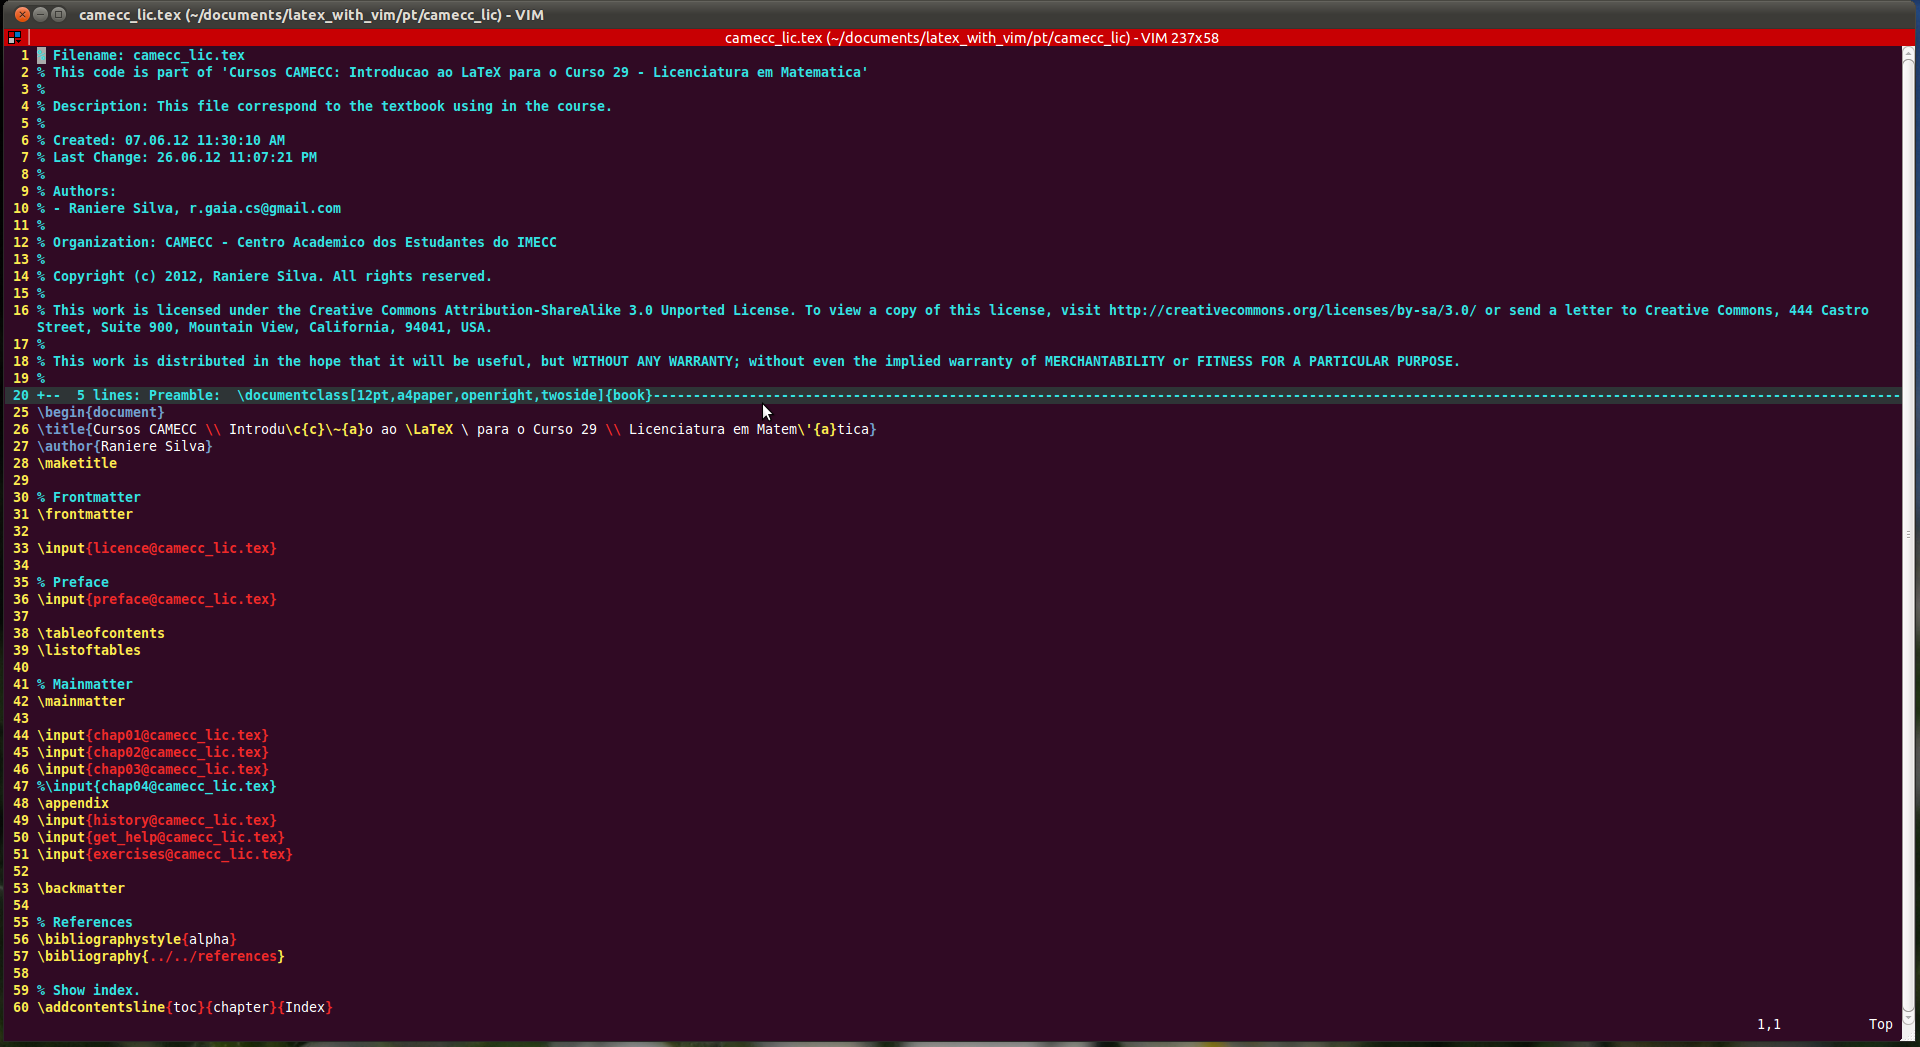
\includegraphics[width=0.4\textwidth]{../../figures/vim.png} &
        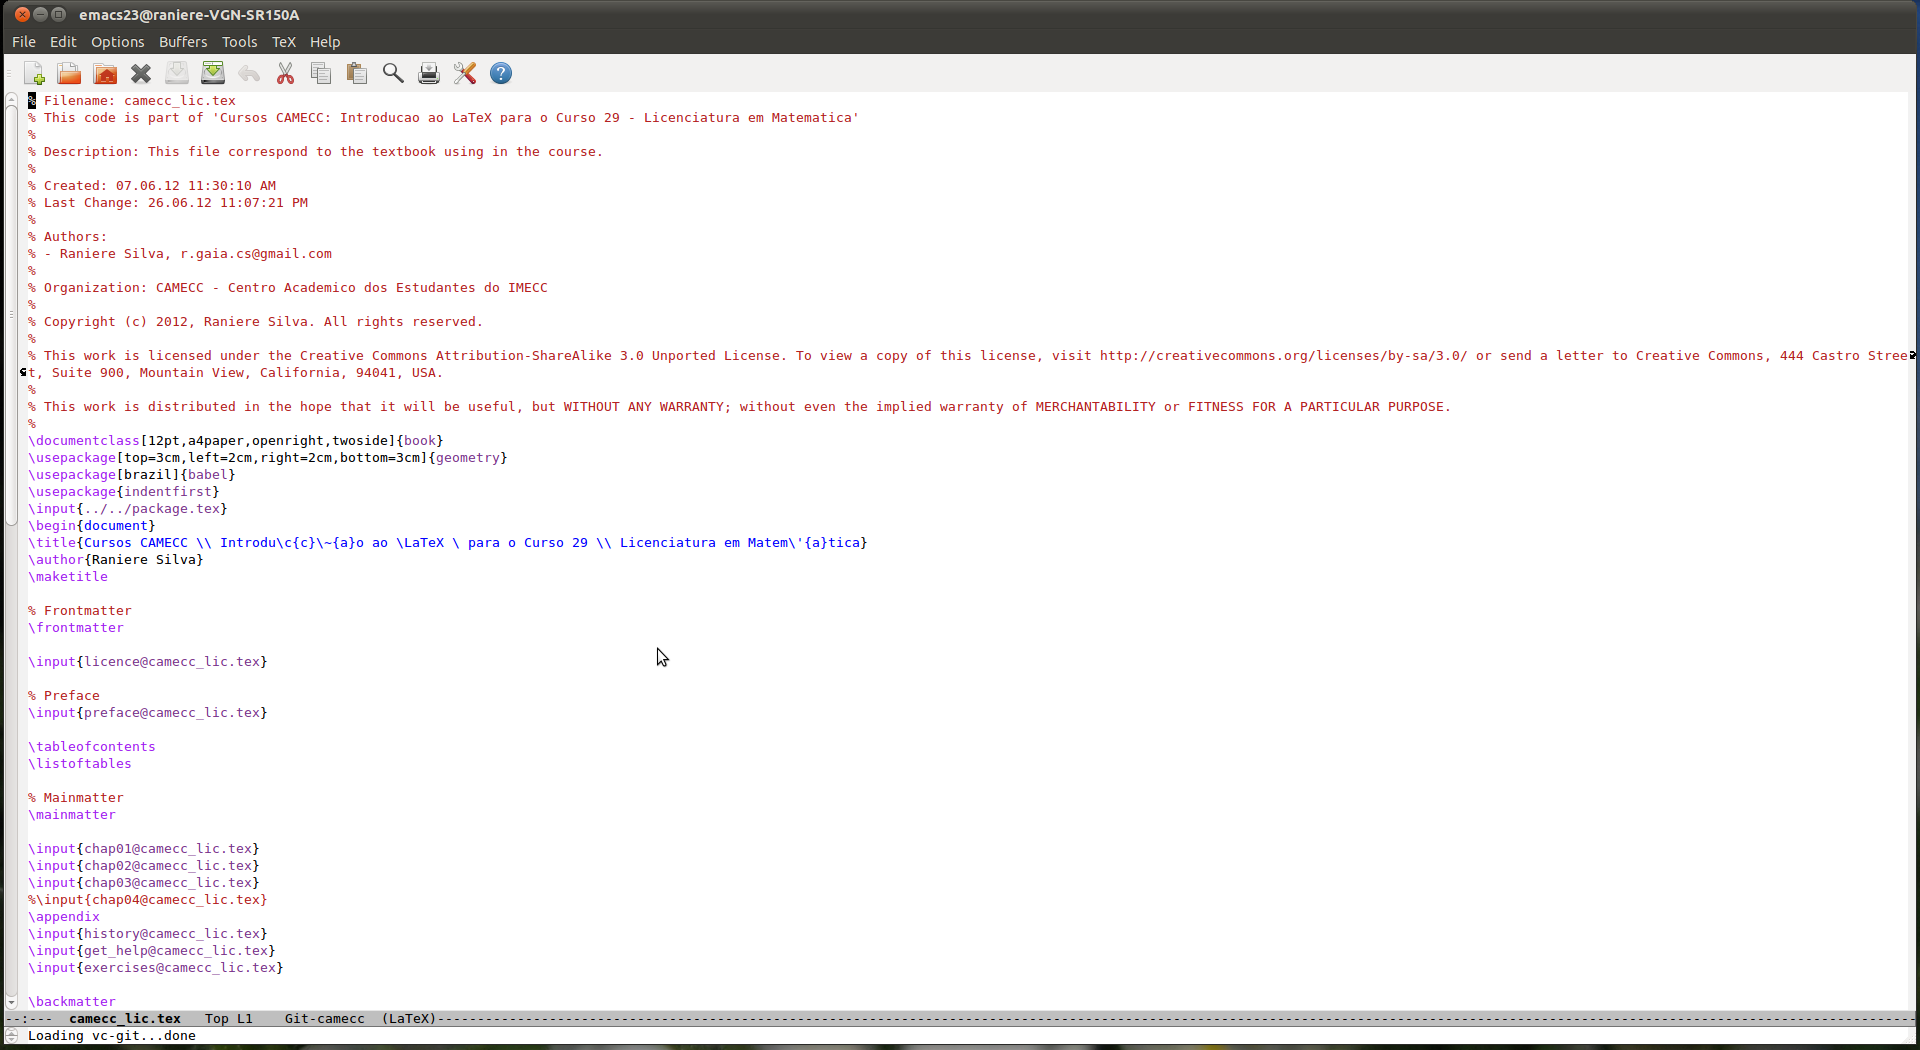
\includegraphics[width=0.4\textwidth]{../../figures/gnu_emacs.png} \\
        Vim & GNU Emacs
    \end{tabular}
    \caption{\flang{Screenshots} de alguns IDE's}
    \label{fig:ide_screenshot}
\end{figure}

\section{Arquivo \lcode{.tex}} \label{sse:basic:tex}
O LaTeX utiliza \lcode{.tex}\index{.tex@\lcode{.tex}} como extensão padrão. O arquivo \lcode{main.tex}, onde \lcode{main} representa o nome do arquivo \lcode{.tex}, é um arquivo de texto, estruturado em duas partes:
\begin{enumerate}
    \item \emph{preâmbulo}\index{preambulo@\emph{pre\^{a}mbulo}}
    \item \emph{informação}\index{informacao@\emph{informa\c{c}\~{a}o}}
\end{enumerate}
sendo que a segunda parte deve ser delimitada pelo ambiente \envname{document}, i.e., ser incluida no lugar de \lcode{XXX} do código abaixo:
\begin{code}
\begin{document}
XXX
\end{document}
\end{code}

\'{E} permito incluir um ou mais arquivo dentro de \lcode{main.tex}, isto é, trabalhar com múltiplos arquivos\index{multiplos arquivos@m\'{u}ltiplos arquivos}. Os arquivos a serem incluídos também possuem a extensão \lcode{.tex} mas devem conter apenas a \emph{informação}.\footnote{Ao trabalhar com múltiplos arquivos apenas precisa-se compilar o arquivo \lcode{main.tex}.}

Uma das forma de incluir um arquivo é com o comando \lstinline!\input!\index{comando!input@\lstinline+\input+}, como ilustrado a seguir:
\begin{code}
\input{aux.tex}
\end{code}
onde \lcode{aux.tex} é o nome do arquivo a ser incluído.\footnote{Caso a extens\~{a}o do arquivo seja suprimida ser\'{a} utilizada \lcode{.tex}.}

Quando \lcode{main.tex} for compilado o arquivo \lcode{aux.tex} será lido e processado exatamente como se tive-se sido inserido na posição que o comando \lstinline!\input! ocupa.

\section{\emph{Preâmbulo}} \label{sse:basic:preamble}
O \emph{preâmbulo}\index{preambulo@\emph{pre\^{a}mbulo}} deve ser iniciado por
\begin{code}
\documentclass[options]{class}
\end{code}
onde \lcode{class}\index{comando!documentclass@\lstinline+\documentclass+} indica o tipo de documento a ser criado e \lcode{options} \'{e} uma lista de palavras chaves separadas por v\'{i}rgula que personaliza o compartamento de \lcode{class} (na Tabela \ref{tab:par_options} encontra-se algumas das palavras chaves disponíveis).
\begin{table}[h!tb]
    \centering
    \caption{Parâmetros disponíveis para \lcode{options}.} \label{tab:par_options}
    \begin{tabular}{llp{0.6\textwidth}}
    \hline
    Função & Código & Descrição \\ \hline
    \multirow{4}{*}{Tamanho} &  & Utiliza, por padrão, o tamanho 10. \\
    & \lcode{10pt} & Tamanho 10. \\
    & \lcode{11pt} & Tamanho 11. \\
    & \lcode{12pt} & Tamanho 12. \\ \hline
    \multirow{7}{*}{Papel} & & Utiliza, por padrão, o tamanho da folha correspondente carta. \\
    & \lcode{letterpaper} & Tamanho da folha correspondente carta. \\
    & \lcode{a4paper} & Tamanho da folha correspondente a A4. \\
    & \lcode{a5paper} & Tamanho da folha correspondente a A5. \\
    & \lcode{b5paper} & Tamanho da folha correspondente a B5. \\
    & \lcode{executivepaper} & Tamanho da folha correspondente a folha executiva. \\
    & \lcode{legalpaper} & Tamanho da folha correspondente a folha legal. \\ \hline
    \multirow{2}{*}{Al. equação} & & Por padrão centra as equações. \\
    & \lcode{fleqn} & Alinha as equações à esquerda. \\ \hline
    \multirow{2}{*}{Nº equação} & & Por padrão enumera as equações à direita. \\
    & \lcode{leqno} & Enumera as equações à esquerda. \\ \hline
    \multirow{4}{*}{Título} & & Por padrão a classe \lcode{article} não começa uma nova página após o título, enquanto que \lcode{report} e \lcode{book} o fazem. \\
    & \lcode{titlepage} & Começa uma nova página após o título. \\
    & \lcode{leqno} & Não começa uma nova página após o título. \\ \hline
    \multirow{4}{*}{Faces} & & Por padrão a classe \lcode{article} e \lcode{report} são a uma face e a classe \lcode{book} é a duas. \\
    & \lcode{oneside} & Gera o documento a uma face. \\
    & \lcode{twoside} & Gera o documento a duas fazes. \\ \hline
    \multirow{5}{*}{Começo} & & Não funciona com a classe \lcode{article} por nesta não existirem capítulos e por padrão a classe \lcode{report} começa os capítulos na próxima página disponível e a classe \lcode{book} sempre nas páginas à direita. \\
    & \lcode{openright} & Começa os capítulos sempre nas páginas à direita. \\
    & \lcode{openany} & Começa os capítulos na próxima página disponível. \\ \hline
    Colunas & \lcode{twocolumn} & Gera o arquivo utilizando-se de duas colunas. \\
    \hline
\end{tabular}

\end{table}

\lcode{class}\index{comando!documentclass@\lstinline+\documentclass+!class@\lcode{class}} corresponde ao nome de um arquivo \lcode{.cls}, os principais são apresentados na Tabela \ref{tab:documentclass} e outros são indicados em \url{http://aprendolatex.wordpress.com/2007/07/15/mais-classes-de-documentos/}. Existe ainda alguns arquivos \lcode{.cls} personalizados disponíveis na internet, destacando-se o \lcode{abnt.cls}, disponível em \url{http://abntex.codigolivre.org.br/}, indicado para documentos que devem seguir as normas da ABNT e o usu\'{a}rio tamb\'{e}m pode escrever sua pr\'{o}pria \lcode{class}.
\begin{table}[h!tb]
    \centering
    \caption{Parâmetros disponíveis para \lcode{class}.} \label{tab:documentclass}
    % Filename: documentclass@latex_with_vim.tex
% This code is part of LaTeX with Vim.
% 
% Description: LaTeX with Vim is free book about Vim, LaTeX and Git.
% 
% Created: 30.03.12 12:12:55 AM
% Last Change: 30.03.12 12:13:08 AM
% 
% Author: Raniere Gaia Costa da Silva, r.gaia.cs@gmail.com
% Organization:  
% 
% Copyright (c) 2010, 2011, 2012, Raniere Gaia Costa da Silva. All rights 
% reserved.
% 
% This file is license under the terms of a Creative Commons Attribution 
% 3.0 Unported License, or (at your option) any later version. More details
% at <http://creativecommons.org/licenses/by/3.0/>.
\begin{tabular}{lp{0.8\textwidth}}
    \hline
    Código & Descrição \\ \hline
    \lcode{article} & Para artigos em revistas especializadas, palestras, trabalhos de disciplinas \dots \\
    \lcode{report} & Para informes maiores que constam de mais de um capítulo, projetos de fim de curso, dissertações, teses e similares. \\
    \lcode{book} & Para livros. \\
    \lcode{slide} & Para transparências. \\
    \lcode{beamer} & Para apresenta\c{c}\~{o}es. \\
    \lcode{exam} & Para lista de exerc\'{i}cios. \\
    \hline
\end{tabular}

\end{table}

O \emph{preâmbulo}\index{preambulo@\emph{pre\^{a}mbulo}} é completado com a inclus\~{a}o de pacotes que serão utilizados na \emph{informação}. O comando para inclus\~{a}o de um pacote\index{comando!usepackage@\lstinline+\usepackage+} segue a seguinte sintaxe:
\begin{code}
\usepackage[options]{package}
\end{code}
onde \lcode{package} é o nome do pacote e \lcode{options} é uma lista de palavras chaves correspondente a op\c{c}\~{o}es do pacote.

Por \'{u}ltimo, \'{e} no \emph{pre\^{a}mbulo} que o usu\'{a}rio tamb\'{e}m pode definir seus pr\'{o}prios comandos e ambientes\footnote{N\~{a}o ser\'{a} abordado neste curso, uma \'{o}tima fonte \'{e} \url{http://en.wikibooks.org/wiki/LaTeX/Customizing_LaTeX}}.

\section{Hello world} \label{sse:basic:hello_world}
Anterioremente foi apresentado os aplicativos necessários para trabalhar com LaTeX e as duas partes principais do arquivo \lcode{.tex}. A seguir apresentaremos como construir a \emph{informação}\index{informacao@\emph{informa\c{c}\~{a}o}}.

O documento mais simples que podemos criar \'{e} apresentado abaixo. \\ 
\begin{minipage}[t]{0.5\linewidth}
    \vspace{-8pt}
    \begin{code}
\documentclass[10pt,a4paper]{article}
\begin{document}
Hello world.
\end{document}
    \end{code}
\end{minipage} \quad \vrule \quad
\begin{minipage}[t]{0.35\linewidth} \vspace{0pt}
    Hello world.
\end{minipage}

Os exemplos que serão apresentados aparecerão seguindo o modelo acima, isto é, em duas colunas sendo a coluna da esquerda contendo o código LaTeX e a coluna da direita contendo a saída obtida. Por simplicidade, nos demais exemplos iremos apresentar apenas a \emph{informação}.

\subsection{Teclado e Idioma}
Na \'{e}poca que o TeX foi desenvolvido utilizava-se a codifica\c{c}\~{a}o ASCII (American Standard Code for Information Interchange) e, consequentemente, o LaTeX foi desenvolvido para utilizar apenas os caracteres presentes na codifica\c{c}\~{a}o ASCII.

As 52 letras (26 letras minúsculas + 26 letras maiúsculas) do alfabeto americano, os dez dígitos indo-arábicos, seis sinais de pontuação (\lstinline+, ; . ? ! :+) e quatro parenteses (\lstinline!( ) [ ]!). Todos estas teclas são interpretadas como elas mesmas pelo LaTeX.

Na seção \ref{sss:basic:space} abordaremos como o LaTeX interpreta o espaço e enter (mudança de linha).

As teclas correspondentes a \lstinline!`!, acento grave, \lstinline!'!, apóstrofe, e \lstinline!-!, hífen, são interpretadas pelo LaTeX de acordo com os caracteres adjacentes.

Os seis símbolos matemáticos (\lstinline!* + = < > /!) são interpretados de maneira diferentes quando no modo texto e no modo matemático\footnote{O modo matemático é apresentado no capítulo \ref{sch:math}.}.

Existem, também, 13 símbolos especiais (\lstinline!# $ % & ~ _ ^ \ { } @ " |!) que são interpretados pelo LaTeX de acordo com os caracteres adjacentes.

Os demais caracteres disponíveis no teclado, quando utilizados, costumam produzir erro.

Para facilitar o uso do LaTeX em outros idiomas que n\~{a}o o ingl\^{e}s pode-se utilizar alguma codificação diferente da ASCII para o arquivo \lcode{.tex}. As codificações mais comuns são UFT-8 e Latin1 sendo que para arquivos codificados com UFT-8 deve-se adicionar a seguinte linha no preâmbulo
\begin{code}
\usepackage[utf8]{inputenc}
\end{code}\index{pacote!inputenc@\pkgname{inputenc}}
enquanto que para arquivos codificados com Latin1
\begin{code}
\usepackage[latin1]{inputenc}
\end{code}
Recomenda-se utilizar a codifica\c{c}\~{a}o UFT-8 (Unicode) pois a Latin1 n\~{a}o possue mais suporte desde 2004 (ver \url{http://pt.wikipedia.org/wiki/ISO_8859-1}) ou apenas os caracteres definidos na codifica\c{c}\~{a}o ASCII pois estes possuem a mesma representa\c{c}\~{a}o na maioria das codifica\c{c}\~{o}es existentes.

É importante que o editor que esteja sendo usado também esteja configurado para trabalhar com a codificação especificada. Quando uma codificação errada estiver sendo usada, o editor pode trocar ou omitir alguns caracteres.

Ao gerar um arquivo pdf utilizando o LaTeX ocorre que copiar e colar um fragmento de texto no pdf com caracteres que n\~{a}o esteja presentes na codifica\c{c}\~{a}o ASCII ser\'{a} preciso corrigir o fragmento. Para atenuar esse trabalho deve-se utilizar o pacote \envname{fontenc}\index{pacote!fontenc@\envname{fontenc}}.

Al\'{e}m disso, deve-se utilizar o pacote \pkgname{babel}\index{pacote!babel@\pkgname{babel}} de Johannes L. Braams que ajusta algumas macros de acordo com o idioma desejado, como a traduções de alguns termos e uso de caixa alta. O pacote \pkgname{babel} que possue as seguintes opções para o idioma português: \lcode{portuges}, \lcode{portuguese}, \lcode{brazil}, \lcode{brazilian}. Maiores detalhes podem ser encontrados na documenta\c{c}\~{a}o do pacote\cite{Braams:2008:Babel}.

\subsection{Espaços, linhas, parágrafos e páginas} \label{sss:basic:space}
No LaTeX o espaço entre palavras apresenta uma particularidade: ele \'{e} ignorado se houver dois ou mais espaços seguidos, como podemos observar a seguir. \\
\example{codes/hello_spaces@latex_with_vim.tex}

Quando for necessário gerar dois ou mais espaços seguidos deve-se utilizar a barra invertida entre os espaços como ilustrado a seguir. \\
\example{codes/hello_spaces_backslash@latex_with_vim.tex}

Nos dois exemplos anteriores é possível verificar que a mudança de linha no código não produz uma nova linha\index{nova linha} no documento gerado. A mudança de linha no LaTeX é representada por \lstinline!\\!\index{comando! @\lstinline+\\+} ou pelo comandos \lstinline!\newline!\index{comando!newline@\lstinline+\newline+}, como ilustrada a seguir. \\
\example{codes/hello_newlines@latex_with_vim.tex}

Já a mudança de parágrafo\index{paragrafo@par\'{a}grafo} é indicada por uma linha em branco. 

Quando for necessário forçar uma mudança de página utiliza-se o comando \lstinline!\newpage!\index{comando!newpage@\lstinline+\newpage+}. Assim como o LaTeX ignora dois ou mais espaços seguidos a mudança de linha e de página também é ignorada.

Por último é importante avisar que, por padr\~{a}o, o primeiro parágrafo de  capítulo, seções, \dots, não é identado. Quando desejar-se identar o primeiro parágrago uma solução é utilizar o pacote \pkgname{indentfirst}.

\subsection{Hifenização}
O LaTeX tenta balancear o tamanho das linhas a serem geradas e para isso utiliza-se de um banco de dados para hifenizar, quando necessário, alguma palavra.

Algumas vezes a hifenização\index{hifenizacao@hifeniza\c{c}\~{a}o} ocorre de maneira inadequada e para corrigir devemos utilizar o comando \lstinline!\hyphenation!\index{comando!hyphenation@\lstinline+\hyphenation+} cujo parâmetro é uma lista de palavras, separadas por espaço, onde o comando - é utilizado para indicar onde a palavra pode ser separada.

\subsection{Acentos}
Embora seja possivel utilizar algumas codifica\c{c}\~{o}es de arquivo que suportam acentua\c{c}\~{a}o utilizando o pacote \pkgname{inputenc} \'{e} importante saber como inserir os acentos utilizando apenas a tabela ASCII que \'{e} apresentado na Tabela~\ref{tab:diacritic}.
\begin{table}[!htb]
    \centering
    \caption{Acentuação (utilizando a vogal ``o'' para exemplo).} \label{tab:diacritic}
    % Filename: diacrict@latex_with_vim.tex
% This code is part of LaTeX with Vim.
% 
% Description: LaTeX with Vim is free book about Vim, LaTeX and Git.
% 
% Created: 30.03.12 12:12:36 AM
% Last Change: 30.03.12 12:12:40 AM
% 
% Author: Raniere Gaia Costa da Silva, r.gaia.cs@gmail.com
% Organization:  
% 
% Copyright (c) 2010, 2011, 2012, Raniere Gaia Costa da Silva. All rights 
% reserved.
% 
% This file is license under the terms of a Creative Commons Attribution 
% 3.0 Unported License, or (at your option) any later version. More details
% at <http://creativecommons.org/licenses/by/3.0/>.
\begin{tabular}{cc|cc|cc|cc}
    \hline
    Comando & Resultado & Comando & Resultado & Comando & Resultado & Comando & Resultado \\ \hline
    \textbackslash '\{o\} & \'{o} & \textbackslash =\{o\} & \={o} & \textbackslash u\{o\} & \u{o} & \textbackslash .\{o\} & \.{o} \\
    \textbackslash v\{o\} & \v{o} & \textbackslash r\{o\} & \r{o} & \textbackslash c\{c\} & \c{c} & \textbackslash t\{oo\} & \t{oo} \\
    \textbackslash \textasciicircum \{o\} & \^{o} & \textbackslash \textasciitilde \{o\} & \~{o} & \textbackslash "\{o\} & \"{o} & \textbackslash d\{o\} & \d{o} \\
    \textbackslash H\{o\} & \H{o} & \textbackslash b\{o\} & \b{o} & \textbackslash `\{o\} & \`{o} & \textbackslash i & \i \\ \hline
\end{tabular}

\end{table}

\section{Caracteres especiais}
No LaTeX alguns caracteres apresentam forma própria de representação. A seguir enunciaremos alguns.

\subsection{Aspas}
Para as aspas\index{aspas} não deve-se usar o caracter de aspas. Para abrir as aspas deve-se utilizar o acento simples e para fechar a aspa simples. \\
\example{codes/quotation_mark@latex_with_vim.tex}

\subsection{Traço}
LaTeX admite três tipos de traço\index{traco@tra\c{c}o}. \\
\example{codes/dashes@latex_with_vim.tex}

\subsection{Pontos sucessivos}
Utiliza-se o comando \lstinline!\dots! ou \lstinline!\ldots! para pontos sucessivos. \\
\example{codes/dots@latex_with_vim.tex}

\subsection{Pontuação e demais símbolos}
Para pontuação\index{pontuacao@pontua\c{c}\~{a}o} e demais símbolos especias deve-se proceder como na Tabela~\ref{tab:symbols}.
\begin{table}[h!tb]
    \centering
    \caption{Para pontuação e símbolos especias.}
    \label{tab:symbols}
    % File: symbols@latex-with-vim.tex
% This code is part of LaTeX with Vim.
% 
% Description: LaTeX with Vim is free book about Vim, LaTeX and Git.
% 
% Created: 30.03.12 12:19:38 AM
% Last Change: 30.03.12 12:19:44 AM
% 
% Author: Raniere Gaia Costa da Silva, r.gaia.cs@gmail.com
% Organization:  
% 
% Copyright (c) 2010, 2011, 2012, Raniere Gaia Costa da Silva. All rights 
% reserved.
% 
% This file is license under the terms of a Creative Commons Attribution 
% 3.0 Unported License, or (at your option) any later version. More details
% at <http://creativecommons.org/licenses/by/3.0/>.

\begin{tabular}{cc|cc|cc}
    \hline
    Comando & Resultado & Comando & Resultado & Comando & Resultado \\ \hline
    \textbackslash \& & \& & \textbackslash textasteriskcentered & \textasteriskcentered & \textbackslash textbackslash & \textbackslash \\
    \textbackslash textbar & \textbar & \textbackslash \{ & \{ & \textbackslash \} & \} \\
    \textbackslash texbullet & \textbullet & \textbackslash textasciitilde & \textasciitilde & \textbackslash textasciicircum & \textasciicircum \\
    \textbackslash copyright & \copyright & \textbackslash textregistered & \textregistered & \textbackslash texttrademark & \texttrademark \\
    \textbackslash textperiodcentered & \textperiodcentered & \textbackslash textexclamdown & \textexclamdown & \textbackslash textquestiondown & \textquestiondown \\
    \textbackslash \% & \% & \textbackslash textgreater & \textgreater & \textbackslash textless & \textless  \\
    \textbackslash \# & \# & \textbackslash S & \S & \textbackslash P & \P \\
    \textbackslash \_ & \_ & \textbackslash dag & \dag & \textbackslash ddag & \ddag \\
    \textbackslash pounds & \pounds & \textbackslash textsuperscript\{a\} & \textsuperscript{a} & \textbackslash textcircled\{a\} & \textcircled{a} \\
    \textbackslash textvisiblespace & \textvisiblespace & \textbackslash \$ & \$ & \textbackslash euro & \euro \\ \hline
\end{tabular}

\end{table}

Destaca-se que para que o símbolo \euro \ seja impresso é necessário que o \emph{preâmbulo} contenha a seguinte linha de código
\begin{code}
    \usepackage[official]{eurosym}
\end{code}

\subsection{Comentários}
Também é possível inserir comentários\index{comentarios@coment\'{a}rios} no arquivo \lcode{.tex}, utilizando-se para isso do caractere \lstinline!%!\index{comando! @\lstinline+%+} de forma que todo o texto posterior ao mesmo e na mesma linha é considerado comentário e não é processado.

\section{Margens}
A configura\c{c}\~{a}o de margens\index{margens} no LaTeX pode ser feita nativamente, utilizando o pacote \pkgname{geometry} ou o pacote \pkgname{fancyhdr}. A seguir abordaremos o pacote \pkgname{geometry} e o estilo de p\'{a}gina.

\subsection{\pkgname{geometry}}
O uso deste pacote é bastante simples, precisa-se apenas fazer a chamada do pacote e atribuir valores para os parâmetros disponíveis. A seguir apresentamos um exemplo:
\begin{code}
\usepackage{geometry}
\geometry{parameter = length, ...}
\end{code}
ou
\begin{code}
\usepackage[parameter = length, ...]{geometry}
\end{code}\index{pacote!geometry@\pkgname{geometry}}

Podemos utilizar \lcode{length} em qualquer unidade disponível no LaTeX, mm, cm e outras. Já as opções para \lcode{parameter} mais utilizadas são apresentadas na Tabela~\ref{tab:par_geometry} e ilustradas na Figura~\ref{fig:par_geometry}.
\begin{table}[h!tb]
    \centering
    \caption{Opções disponíveis para \lcode{parameter}, referente ao pacote \lcode{geometry}.}
    \label{tab:par_geometry}
    % File: geometry@latex-with-vim.tex
% This code is part of LaTeX with Vim.
% 
% Description: LaTeX with Vim is free book about Vim, LaTeX and Git.
% 
% Created: 30.03.12 12:19:38 AM
% Last Change: 30.03.12 12:19:44 AM
% 
% Author: Raniere Gaia Costa da Silva, r.gaia.cs@gmail.com
% Organization:  
% 
% Copyright (c) 2010, 2011, 2012, Raniere Gaia Costa da Silva. All rights 
% reserved.
% 
% This file is license under the terms of a Creative Commons Attribution 
% 3.0 Unported License, or (at your option) any later version. More details
% at <http://creativecommons.org/licenses/by/3.0/>.

\begin{tabular}{lp{0.8\textwidth}}
    \hline
    Código & Descrição \\ \hline
    \lcode{paperwidth} & Largura do papel. \\
    \lcode{paperheight} & Altura do papel. \\
    \lcode{textwidth} & Largura da caixa de texto. \\
    \lcode{textheigth} & Altura da caixa de texto. \\
    \lcode{top} & Margem superior. \\
    \lcode{bottom} & Margem inferior. \\
    \lcode{lefth} & Margem esquerda. \\
    \lcode{right} & Margem direita. \\ \hline
\end{tabular}

\end{table}
\begin{figure}[h!]
    \centering
    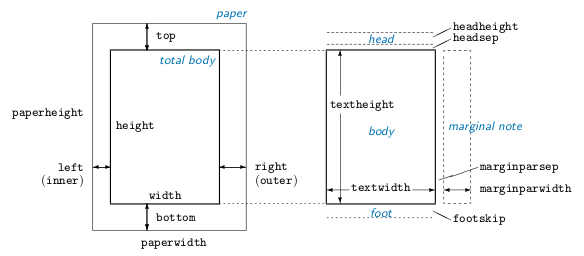
\includegraphics[width=0.8\textwidth]{figures/geometry_margin.png}
    \flushright Fonte: \cite{Umeki:2010:Geometry}
    \caption{Ilustração da opções disponíveis para \lcode{parameter} apresentadas na Tabela \ref{tab:par_geometry}.} \label{fig:par_geometry}
\end{figure}

\subsection{Estilo de p\'{a}gina}

Existe um estilo de página definido como padrão\footnote{Corresponde ao estilo \lcode{plain} apresentado na Tabela \ref{tab:par_style}.}, quando deseja-se mudar o estilo em todo o documento pode-se utilizar o comando
\begin{code}
\pagestyle{style}
\end{code}
e quando for necessário mudá-lo apenas na página atual utiliza-se o comando
\begin{code}
\thispagestyle{style}
\end{code}

As opções para \lcode{style} são apresentadas na Tabela~\ref{tab:par_style}.
\begin{table}[!htb]
    \centering
    \caption{Opções disponíveis para \lcode{style}.}
    \label{tab:par_style}
    % File: style@latex-with-vim.tex
% This code is part of LaTeX with Vim.
% 
% Description: LaTeX with Vim is free book about Vim, LaTeX and Git.
% 
% Created: 30.03.12 12:19:38 AM
% Last Change: 30.03.12 12:19:44 AM
% 
% Author: Raniere Gaia Costa da Silva, r.gaia.cs@gmail.com
% Organization:  
% 
% Copyright (c) 2010, 2011, 2012, Raniere Gaia Costa da Silva. All rights 
% reserved.
% 
% This file is license under the terms of a Creative Commons Attribution 
% 3.0 Unported License, or (at your option) any later version. More details
% at <http://creativecommons.org/licenses/by/3.0/>.

\begin{tabular}{lp{0.8\textwidth}}
    \hline
    Código & Descrição \\ \hline
    \lcode{plain} & Imprime os números de página no centro do pé da página. \\
    \lcode{headings} & No cabeçalho de cada página imprime o capítulo que está sendo processado e o número da página. O pé da página fica vazio. \\
    \lcode{empty} & Coloca tanto o cabeçalho como o pé da página vazios.
\end{tabular}

\end{table}

Aos interessados em criar um estilo próprio, sugere-se utilizar o pacote \lcode{fancyhdr}.
\section{Fonte}
No LaTeX estão disponíveis algumas fontes\index{fonte} opcionais. Comandos da forma \lstinline!\textXX! são responsáveis por alterar a fonte sendo que \lcode{XX} corresponde ao código da fonte a serem utilizados. A Tabela~\ref{tab:text} apresenta alguns das opções disponíveis.
\begin{table}[!htb]
    \centering
    \caption{Opções disponíveis para \lcode{XX} da fonte.} \label{tab:text}
    % Filename: text@latex_with_vim.tex
% This code is part of LaTeX with Vim.
% 
% Description: LaTeX with Vim is free book about Vim, LaTeX and Git.
% 
% Created: 30.03.12 12:19:02 AM
% Last Change: 30.03.12 12:19:06 AM
% 
% Author: Raniere Gaia Costa da Silva, r.gaia.cs@gmail.com
% Organization:  
% 
% Copyright (c) 2010, 2011, 2012, Raniere Gaia Costa da Silva. All rights 
% reserved.
% 
% This file is license under the terms of a Creative Commons Attribution 
% 3.0 Unported License, or (at your option) any later version. More details
% at <http://creativecommons.org/licenses/by/3.0/>.
\begin{tabular}{lp{0.8\textwidth}}
    \hline
    Código & Descrição \\ \hline
    \lcode{it} & Texto em itálico. \\
    \lcode{bf} & Texto em negrito. \\
    \lcode{rm} & Texto em romano. \\
    \lcode{sf} & Texto em sans serif. \\
    \lcode{tt} & Texto na tipografia de uma máquina de escrever. \\
    \lcode{sc} & Texto em caixa alta. \\ \hline
\end{tabular}

\end{table}

A seguir é ilustrado as opções apresentadas na Tabela~\ref{tab:text}. \\
\example{codes/hello_fonte@latex_with_vim.tex}

\subsection{Tamanho}
Uma das maneiras de mudar o tamanho da fonte\index{fonte!tamanho} em uma parte do texto é utilizando um dos ambiente  ou comando de tamanho (a Tabela \ref{tab:op_tamanho_fonte} apresenta algumas opções disponíveis).
\begin{table}[h!tb]
    \centering
    \caption{Opções disponíveis para o tamanho da fonte, em ordem crescente.}
    \label{tab:op_tamanho_fonte}
    % Filename: font_size@latex_with_vim.tex
% This code is part of LaTeX with Vim.
% 
% Description: LaTeX with Vim is free book about Vim, LaTeX and Git.
% 
% Created: 30.03.12 12:12:36 AM
% Last Change: 30.03.12 12:12:40 AM
% 
% Author: Raniere Gaia Costa da Silva, r.gaia.cs@gmail.com
% Organization:  
% 
% Copyright (c) 2010, 2011, 2012, Raniere Gaia Costa da Silva. All rights 
% reserved.
% 
% This file is license under the terms of a Creative Commons Attribution 
% 3.0 Unported License, or (at your option) any later version. More details
% at <http://creativecommons.org/licenses/by/3.0/>.
\begin{tabular}{lp{0.7\textwidth}}
    \hline
    Código & Descrição \\ \hline
    \lstinline!\tiny! & O menor tamanho possível. \\
    \lstinline!\SMALL! ou \lstinline!\scriptsize! &  \\
    \lstinline!\Small! ou \lstinline!\footnotesize! & Tamanho utilizado em notas de rodapé. \\
    \lstinline!\small! &  \\
    \lstinline!\normalsize! & Tamanho padrão. \\
    \lstinline!\large! & \\
    \lstinline!\Large! & \\
    \lstinline!\LARGE! & \\
    \lstinline!\huge! & \\
    \lstinline!\Huge! & O maior tamanho disponível. \\ \hline
\end{tabular}

\end{table}

Destaca-se que os tamanhos são baseados no tamanho padrão. A seguir um exemplo. \\
\example{codes/hello_size@latex_with_vim.tex}

\subsection{Cor}
Para alterar a cor\index{fonte!cor} do texto é necessário os pacotes \pkgname{graphicx}\index{pacote!graphicx@\pkgname{graphicx}} e \pkgname{color}\index{pacote!color@\pkgname{color}} e pode-se utilizar um dos comandos: \lstinline!\textcolor!\index{comando!textcolor@\lstinline+\textcolor+} ou \lstinline!\color!\index{comando!color@\lstinline+\color+}.

A seguir apresentamos um exemplo. \\
\example{codes/hello_color@latex_with_vim.tex}

\subsection{Edição direta}
Algumas vezes deseja-se inserir um texto que não deve ser interpretado. Isso é possível pelo ambiente \envname{verbatim}\index{ambiente!verbatim@\envname{verbatim}}, coloca o texto em uma nova linha, e pelo comando \lstinline!\verb!\index{comando!verb@\lstinline+\verb+}, coloca o texto no mesmo parágrafo.

Tanto o ambiente \lcode{verbatim} como o comando \lstinline!\verb! apresentam uma fonte própria. \\
\example{codes/hello_verb@latex_with_vim.tex}

Vale destacar que o comando \textbackslash\lcode{verb} é ``flexível'' quando ao delimitador, os caracteres \lstinline+!+, \lstinline!+! e \lstinline!:! normalmente exercem satisfatoriamente esta função.

\section{Espaçamento}
Nesta seção abordaremos como inserir espaços\index{espa\c{c}os em branco} ao longo do texto no LaTeX, mas antes é importante destacar que podemos suprimir espaços ao utilizar medidas negativas.

\subsection{Espaçamento horizontal}
Para produzir um espaço horizontal utiliza-se o comando \lstinline!\hspace!\index{comando!hspace@\lstinline+\hspace+} que tem como parâmetro o tamanho do espaço a ser inserido. Se o comando ocorrer entre duas linhas ou no início de uma linha o LaTeX não produz o espaço e para este caso devemos utilizar  \lstinline!\hspace*!.

Para modificar a identação característica de um novo parágrafo deve-se utilizar o comando
\begin{code}
\setlength{\parident}{tam}
\end{code} 
onde \lcode{tam} é o novo tamanho para a identação dos parágrafos. No caso de desejar-se suprimir a identação deve-se utilizar o comando \lstinline!\noindent!.

O comando \lstinline!\hfill! cria um espaço suficiente para dividir o texto de modo que o que estiver antes do comando é alinhado a esquerda e o que estiver depois é alinhado a direita. É permitido utilizar o comando mais de uma vez em uma linha. O comando é ignorado quando ocorrer entre duas linhas ou no início de uma linha, neste caso devemos utilizar \lstinline!\hfill*!.

\subsection{Linha horizontal}
Os comandos \lstinline!\dotfill! e \lstinline!\hrulefill! funcionam de maneira semelhante ao comando \lstinline!\hfill!, mas ao invés de inserir um espaço em branco é introduzido, respectivamente uma linha pontilhada e uma linha contínua.

\subsection{Espaçamento vertical}
No capítulo anterior informamos como mudar de linha, nesta seção vamos trabalhar com o espaço entre as linhas.

O comando \lstinline!\baselineskip[tam]! estabelece o tamanho do espaçamento entre linhas para o texto posterior ao comando. Para modificar o tamanho entre duas linhas específicas pode-se utilizar o comando \lstinline!\\[tam]! inicia uma nova linha de maneira que \lcode{tam} é o espaçamento entre as linhas.

Para aumentar o espaço entre parágrafos pode-se utilizar um dos comandos \lstinline!\smallskip!, \lstinline!\medskip! ou \lstinline!\bigskip!, sendo que o tamanho do espaço está relacionado com o tamanho da fonte padrão do documento.

Os comandos \lstinline!\vspace!\index{comando!vspace@\lstinline+\vspace+} e \lstinline!\vfill! funcionam, respectivamente, de modo muito semelhante aos comandos \lstinline!\hspace! e \lstinline!\hfill! só que na vertical.

\subsection{Linha verticais}
O comando \lstinline!\vrule! produz uma linha vertical.

\section{Alinhamento}
Por padrão, o alinhamento\index{alinhamento} ocorre com a margem esquerda e para alterá-lo pode-se utilizar um dos seguintes ambientes: \envname{center} (para texto centralizado), \envname{flushleft} (alinhamento a esquerda) e \envname{flushright} (alinhamento a direita). \\
\example{codes/align@latex_with_vim.tex}

Também é permitido utilizar os comandos: \lstinline!\centering! (para texto centralizado), \lstinline!\raggedleft! (alinhamento a esquerda) e \lstinline!\raggedright! (alinhamento a direita).
